% ===================================================================== % sections/data.tex — shared (long + short) % =====================================================================

\section{Data} \label{sec:data}

\subsection{The Indonesia Family Life Survey}

The analysis uses all five waves of the Indonesia Family Life Survey (IFLS), an ongoing longitudinal household survey conducted between 1993 and 2014. The IFLS sample is representative of approximately 83 percent of the Indonesian population and originally covered roughly \num{30000} individuals in 13 of the country's 27 provinces \autocite{strauss2016}. Re-contact rates across waves are unusually high for a long panel: 94 percent of wave-1 households were reinterviewed in wave 2, and \textcite{thomas2000} document that attrition over the first three waves was largely uncorrelated with baseline observables that predict outcomes. \textcite{ahsan2021} report that 23 percent attrition over thirty years does not threaten identification in the village-midwife setting; in the present analysis sample, attrition since wave 1 is 21 percent and is uncorrelated with the timing of village-midwife arrival.

Three IFLS modules are central to the analysis. The Service Availability Roster (SAR), administered to community informants in waves 2--5, records the type, opening year, and operating status of every health facility serving each community. The community-government (PKK) module independently asks village leaders whether a midwife is present and, if so, in what year she first arrived. Together these two modules yield two parallel measures of program rollout that I describe in Section~\ref{sec:empirical}. Individual-level demographic and outcome data come from the household questionnaire (Books AR, US, 3A, 3B, EK).

\subsection{Sample construction}

Treatment is assigned at the level of an individual's community of birth. Because IFLS does not record birthplace directly, the analysis frame preserves three reconstructions so that downstream specifications can compare them: (i)~a non-mover variant, following \textcite{cas2012} and \textcite{ahsan2021}, that restricts to children whose own community identifier is unchanged across all four waves; (ii)~a variant that instead assigns the mother's community at the wave nearest preceding the child's birth; and (iii)~a variant that restricts on the mother's never-mover status rather than the child's. The three variants yield analytic samples of \NPrimary, roughly \num{10600}, and \num{5638} individuals respectively. The headline analysis uses the non-mover variant: it guarantees a clean birthplace identifier at the cost of dropping children whose families moved across waves. The preceding-wave and mother-never-mover variants are reported in the robustness columns of Table~\ref{tab:robustness}.

The headline sample includes the \NPrimary~non-mover individuals born in 1984--1999 (aged 15--30 in 2014) who are alive at wave~5 across \NVillages~communities. Internal migration was substantial over the relevant period, with rural-to-urban migration moving from 17 to 31 percent of the population between 1971 and 1990 \autocite{alatas1993}; the non-mover restriction therefore selects a sub-sample on which the birthplace-identifier concern is minimised, and the robustness columns on the preceding-wave and mother-never-mover variants assess whether the qualitative patterns survive on the samples that admit internal migration.

Table~\ref{tab:descriptives} reports descriptive statistics for the analysis sample.

\begingroup
\setlength{\tabcolsep}{4pt}
\renewcommand{\arraystretch}{0.95}
\small
\begin{table}
\centering
\caption{Descriptive statistics (primary sample).}
\centering
\begin{tabular}[t]{lrrrr}
\toprule
\multicolumn{1}{c}{ } & \multicolumn{2}{c}{Exposed} & \multicolumn{2}{c}{Control} \\
\cmidrule(l{3pt}r{3pt}){2-3} \cmidrule(l{3pt}r{3pt}){4-5}
  & Mean & SD & Mean & SD\\
\midrule
Female & 0.486 & 0.500 & 0.508 & 0.500\\
Age in 2014 (years) & 22.661 & 2.633 & 22.449 & 4.512\\
Birth year & 1991.339 & 2.633 & 1991.551 & 4.512\\
Mother's education (years) & 5.240 & 3.785 & 5.863 & 3.943\\
Mother's age at birth (years) & 26.674 & 6.689 & 27.020 & 6.455\\
Child height (cm) & 158.375 & 8.815 & 158.194 & 8.126\\
Word-recall score & 530.354 & 61.714 & 530.357 & 58.534\\
CESD-10 depression score (raw) & 7.035 & 4.667 & 7.199 & 4.766\\
Health index (std.) & -0.031 & 0.971 & 0.034 & 0.980\\
Cognition index (std.) & -0.045 & 1.042 & 0.013 & 0.990\\
Depression index (std., higher = better) & 0.032 & 0.981 & -0.002 & 1.001\\
Socioemotional index (std.) & 0.015 & 0.999 & 0.003 & 1.003\\
\bottomrule
\multicolumn{5}{l}{\rule{0pt}{1em}VM = village midwife. See Section text for sample definition.}\\
\end{tabular}
\end{table}

\endgroup
\label{tab:descriptives}

\subsection{Outcome measures}

The analysis collapses outcomes into four families. Each is summarized by a single inverse-covariance-weighted composite index following \textcite{anderson2008}, with raw items retained for sensitivity analysis. By convention, signs are oriented so that higher values of each index indicate a better outcome.

\paragraph{Health.} The health index combines six wave-5 measurements: standing height in centimeters, an indicator for not being underweight (BMI $\geq 18.5$), log-transformed peak expiratory flow, an indicator for not having hypertension, a retrospective indicator for good early-life health, and a self-rated general health rating (re-coded so higher is better).

\paragraph{Cognition.} The cognition index combines wave-5 adult cognitive measures from Book~3B: the IRT-scored adaptive number-series score, the serial-7 subtraction count, and immediate and delayed word-recall counts. The adult IRT score covers the entire 1984--1999 cohort; an alternative child Raven score from Book~EK is administered only to respondents aged 7--14 at wave~5 and is used only in the robustness analysis in Section~\ref{sec:robustness}.

\paragraph{Depression.} The depression index is the standardised sum of the ten CESD-10 items administered in the IFLS wave-5 adult module, sign-flipped so that higher values mean fewer depressive symptoms.

\paragraph{Socioemotional traits.} The socioemotional index averages five trait scores constructed from the fifteen Big-Five Inventory items in the IFLS wave-5 adult module; each trait score is standardised within the wave-5 sample.

Figure~\ref{fig:rollout} shows the distribution of village-midwife rollout years across the \NVillages~communities in the analysis sample, with the program-launch year (1989) and the onset of the Asian Financial Crisis (1997) marked.

\begin{figure}[!htbp] \centering 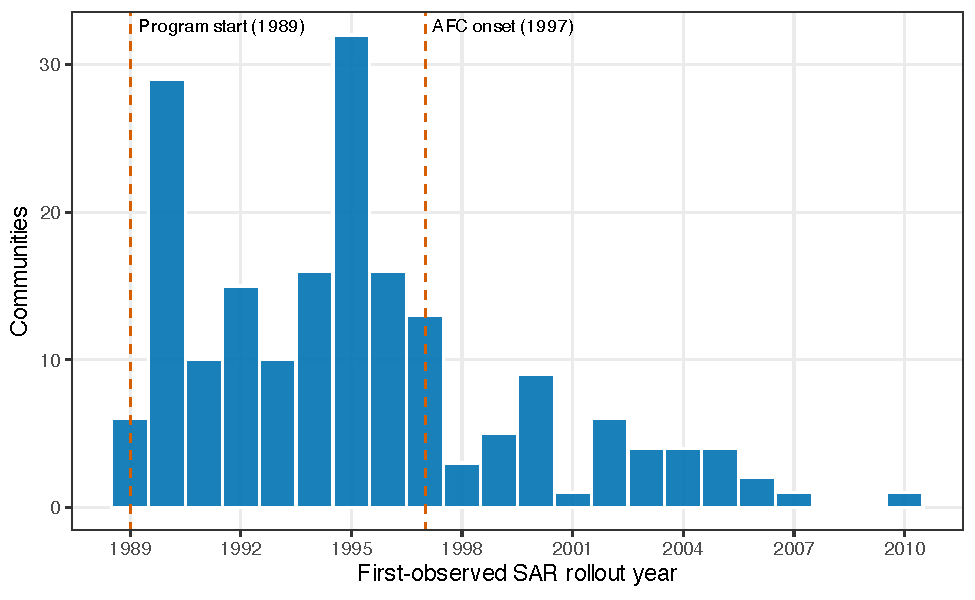
\includegraphics[width=0.9\textwidth]{figures/rollout_histogram.pdf} \caption{Distribution of SAR-recorded village-midwife rollout years across communities in the analysis sample.} \label{fig:rollout} \end{figure}
